\chapter{State Estimation}\label{cha3}
In this chapter is first an introduction in the Kalman Filter and the modified version called Extendend Kalman Filter given. In a second step will the state estimation algorithm, developed during this thesis explained. This gives an overview over the whole code and describes how the parameters were set and how a sensor data outage is handled. Section \ref{state_estimation} and \ref{sensor_estimation} will focus on the two essential parts of the algorithm, how the states are estimated and how the measurements are estimated.
\section{Extended Kalman Filter}

\subsection*{Discrete Kalman Filter}
We will first give a short introduction to the Kalman Filter in general and its mathematical justification.
\begin{quote}The Kalman filter is an extremely effective versatile procedure for combining noisy sensor outputs to estimate the state of a system with uncertain dynamics.\end{quote} […angu...] It was published in 1960 by R.E.Kalman. The Filter gained a strong impact in the area of autonomous or assisted navigation [..pap...]. 
Systems in which the filter is estimating the state $x \in R^{n}$ can be described by the following linear stochastic difference equation.
\begin{equation}
x_{k+1}=A_k*x_k+B_k*u_k+w
\label{eq1}
\end{equation} The next equation shows the relation between the state and the measurement $z \in R^{n}$.
\begin{equation} 
z_k=H_k*x_k+D_k*u_k+v
\label{eq2}
\end{equation}
Where the random variables $w$ and $v$ stand for the process and the measurement noise, which are assumed to be independent, white and normal probability distributions.
\begin{quote}The $n\times n$ matrix A in equation \ref{eq1} relates the state at time step $k$ to the state at step $k+1$, in the absene of either a dirving function or process noise. The $n\times l$ matrix $B$ relates the control input $u \in R^{l}$ to the state $x$. The $m \times m$ matrix $H$ in the measurement equation \ref{eq2} relates to the state to the measurement $z_k$.\end{quote}[.pap.]
In most navigation applications, the noisy sensors are a GPS receiver and an inertial navigation system or other sensors like for example speed sensors. The states of a system are described by the position, velocity, attitude and attitude rate [.angu..].

\subsection*{Mathematical Background}\label{math_kalman}
In figure \ref{simple_schematic} the structure of the algorithm is sketched for a better understanding of the filter's mathematical background. 
\begin{figure}[h]
\begin{center}
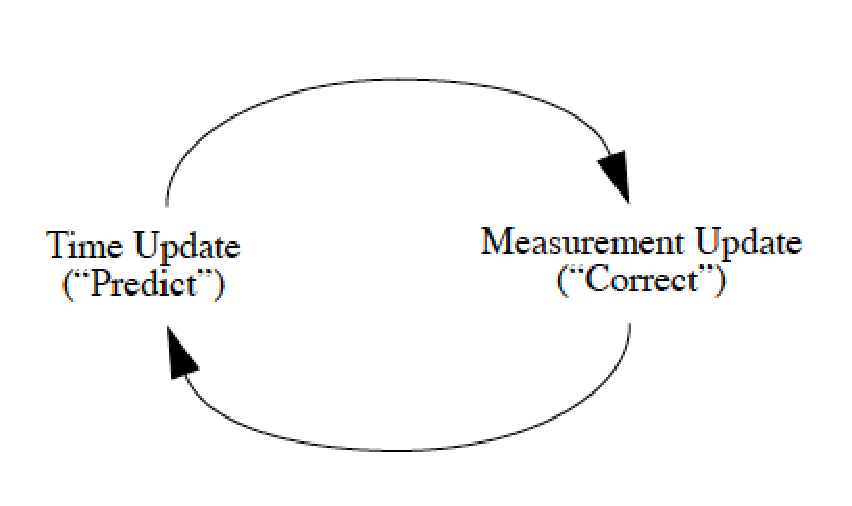
\includegraphics[width=6cm]{pictures/simple_schematic_algo.eps}
\caption{A simple structure of the algorithm}
\label{simple_schematic}
\end{center}
\end{figure}
In a first step the state at $k+1$ is estimated based on \ref{eq1}. This estimation is called a priori state estimation and written as $\hat{x}_k^{-}$. In a second step the a priori state estimation is corrected by the knowledge of measurements $z_k$. This corrected estimation is called the a posteriori estimation and written as $\hat{x}_k$.

Now two error can be defined with it's a error covariances. First the error of the a priori estimation 
\begin{equation}
e^{-}=x_k-\hat{x}_k^{-}
\end{equation}
and second the error of the a posteriori estimation 
\begin{equation}
e=x_k-\hat{x}_k
\end{equation}
with the a priori estimate error covariance 
\begin{equation}
P^{-}_k=E[e^{-}e^{-T}]
\end{equation}
and the a posteriori error covariance.
\begin{equation}
P_k=E[ee^{T}]\label{P_post}
\end{equation}

The Kalman Filter is calculating the a posteriori estimation, the one we are finally looking for. This calculation is a linear combination between the a priori estimated state and the difference of the the estimated measurement $x_k*H$ and the actual measurement $z_k$ weighted with the Kalman gain $K$. This difference $z_k-H_k\hat{x}^{-}_k$ is  called residual and tells us how accurate the estimation of the measurements is. This is summarized in equation \ref{eq7}.
\begin{equation}
\hat{x}_k^{-}*K*(z_k-H_k\hat{x}^{-}_k)\label{eq7}
\end{equation}
The Kalman gain $K$ is the heart of the Kalman Filter. $K$, a $n\times n$ Matrix is chosen in a way to minimize the a posteriori error covariance shown in equation \ref{P-post}. With some calculations the following 
\begin{equation}
K=\frac{P^{-}_k*H^{T}_k}{(H_k*P^{-}_k*H^{T}_k+R_k)}
\end{equation}
can be derived for the Kalman gain $K$.[..pap..]] 
This concept uses the information of a normal gaussian distribution of the noise mentioned in (..equ2..). $P_k$ is minimized using the Maximum Likelihood Estimation and is called the  Gaussian Maximum-Likelihood Estimator […]. A more detailed derivation of the mathematics is shown in [..maybeck..] and [..angu..].

\subsection*{Algorithm}
With equations described in the section above, the estimation and correction step can be summarized as shown in figure \ref{equation_kalman}.
\begin{figure}[h]
\begin{center}
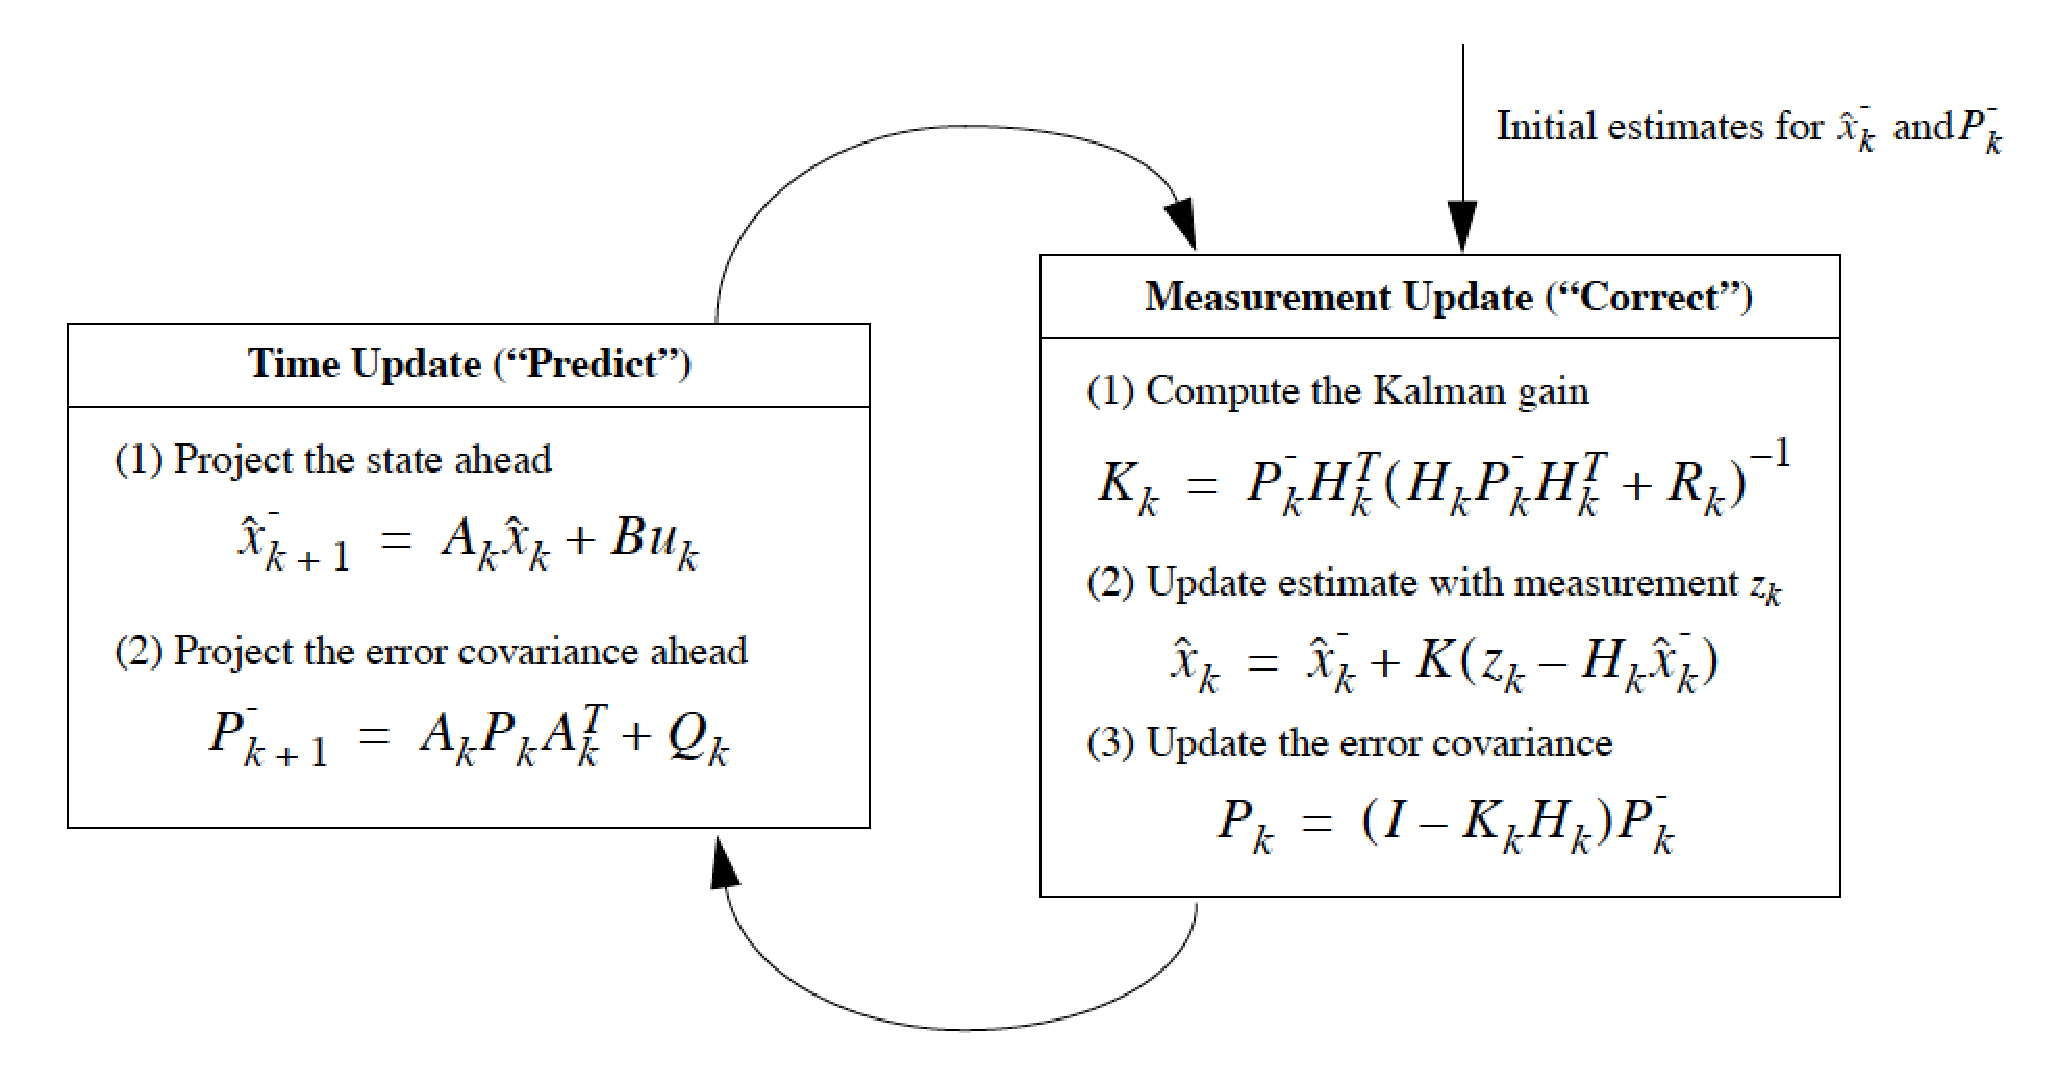
\includegraphics[width=10cm]{pictures/equation_kalman.eps}
\caption{The prediction and the correction step with their corresponding equations. }
\label{equation_kalman}
\end{center}
\end{figure} 
For a fine tuning of the filter often the measurement error covariance matrix $R_k$ and process noise $Q_k$ can be used. $R_k$ contains the information how accurate the sensors and therefore the measurements are expected to be. This can be estimated in a first round with some static sensor test or can be found in the data sheets of the sensors. The matrix $Q_k$ describes how correct the propagation model described by the matrix $A_k$ is believed to be. In this sense as higher the values and therefore the noise of $R_k$ and $Q_k$ the less influence do the measurements or the propagation model respectively have on the estimated state. Having a diagonal matrix with constant values over time, does not represent the reality, but brings it to a form which is fast stable and easier tunable[..pap..]. 

\subsection*{Extended Kalman Filter (EKF)}\label{ekf}
In reality the process to estimate the new state and the measurement relationship to the process is non-linear.
\begin{equation}
x_{k+1}=f(x_k,u_k,w)
z_k=h(x_k,v_k)
\end{equation}
One of the solution to overcome this problem is the Extended Kalman Filter shortly EKF. The EKF is linearizing the this functions with a first order Taylor-Series around the current state. This can be summerized with the following equation:
\begin{equation}
x_{k+1}\approx \hat{x}_{k+1}+A(x_k-\hat{x}_k)+w\\
z_k\approx \hat{z}_k+H(x_k-\hat{x}_k) +v 
\end{equation}
Where $A$ and $H$ are the Jacobian matrix of the function $f$ and $h$.
\begin{equation}
A_{i,j}=\frac{\partial f_{i}}{\partial x_j}(\hat{x}_k,u_k,9)\\
H_{i,j}=\frac{\partial h_{i}}{\partial x_j}(\hat{x}_k,u_k,9)
\end{equation}
This brings us to the summarized equations of the EKF in figure \ref{equation_ekf}.
\begin{figure}[h]
\begin{center}
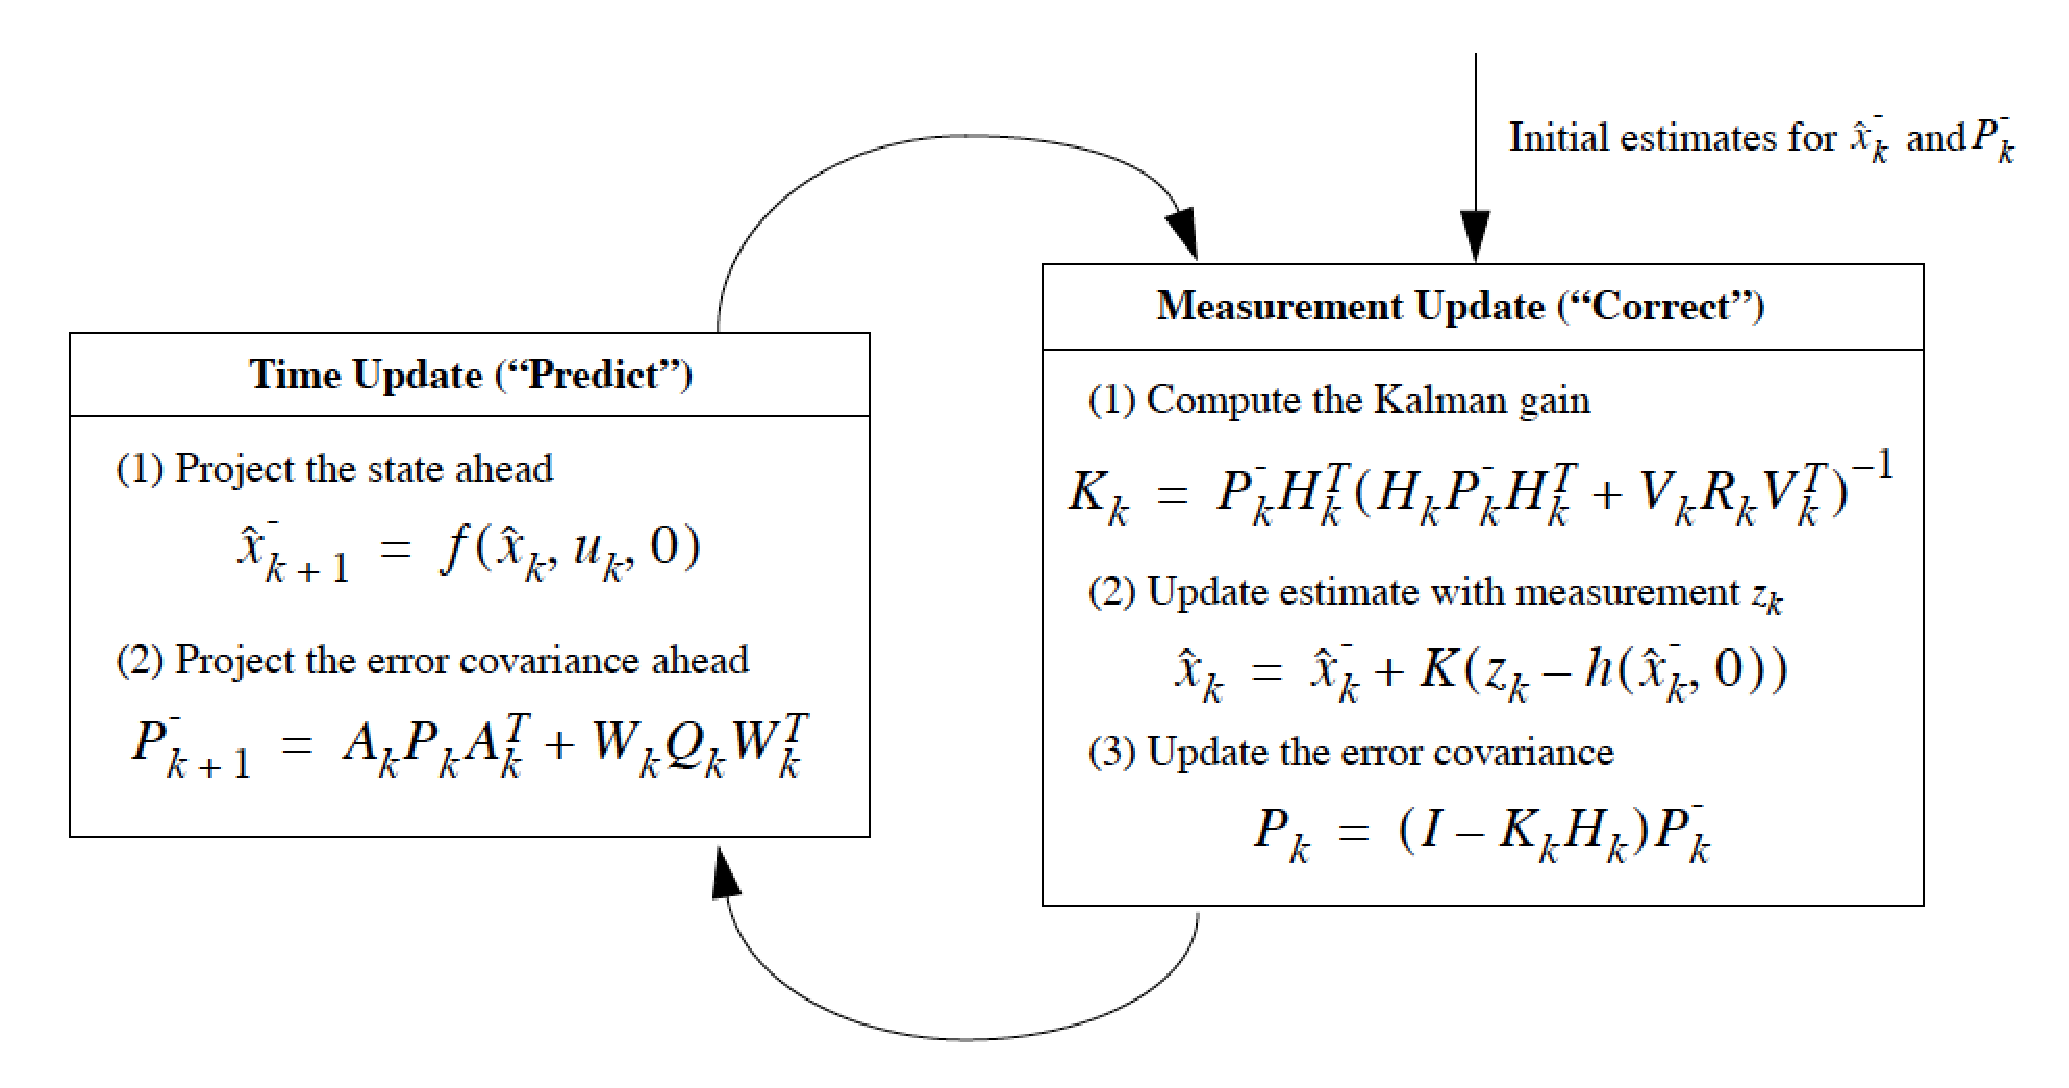
\includegraphics[width=10cm]{pictures/equation_ekf.eps}
\caption{The prediction and correction step of the EKF with their corresponding equations. }
\label{equation_ekf}
\end{center}
\end{figure}


\section{Algorithm for State Estimation}
In this chapter we will present the structure of the state estimation algorithm as we implemented it in MATLAB. As mentioned before, the goal is to get an estimation of the system's state as precise as possible using an Extended Kalman Filter. The Algorithm can be split in several main tasks. First the physical relations between the state $x_{k}$ and the state $x_{k+1}$ has to be defined and summarized in a propagation model. This is needed to calculate the a priori state estimation as described in chapter \ref{math_kalman}. Since this step is  crucial for the accuracy of the algorithm, it is further explained in chapter \ref{state_estimation}. A second key role plays the measurement estimation which corrects the a priori state estimation and calculates the a posteriori state estimation. A more detailed explanation of this correction can be found in chapter \ref{sensor_estimation}. A third question to be elaborated is how the algorithm has to behave if no sensor data is available or if not all sensors provide their outputs with the same frequency. In the last paragraph we will explain how the error covariances were chosen.

\subsection*{Orientation}
The filter has to handle two different coordinates frames. One is the inertial frame and the other the body frame. The inertial frame is the global frame. The position and the velocity both provided by the GPS are in the inertial frame. The origin of the inertial frame lies at the suspension point of the pendulum/kite. The body frame is a coordinate system on the kite. Its z-axis always points in the direction of the line and its origin lies at the center of gravity of the kite. The sensor measurements from the IMU are all in the body frame. Figure \ref{dof} contains an illustration of these two coordinate systems. 

 \begin{figure}[h]
\begin{center}
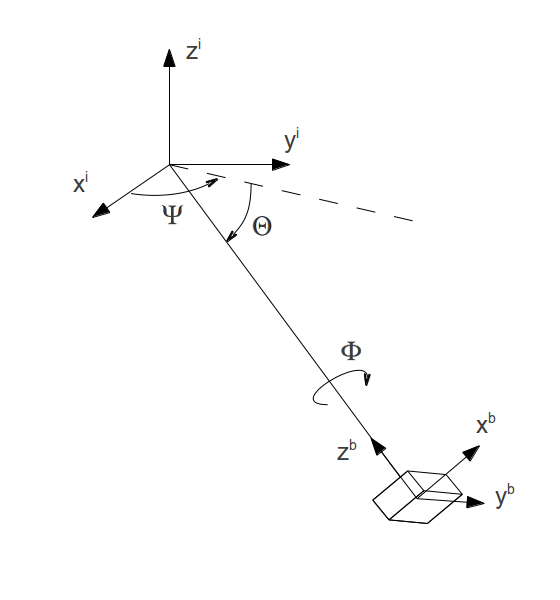
\includegraphics[width=10cm]{pictures/sketch_coordinate_systems.png}
\caption{The definition of the inertial and body frame as well as the convention for the angles in the pendulum model.}
\label{dof}
\end{center}
\end{figure}

The euler angles describe how the inertial frame has to be rotated to bring into the body frame. With other words, the euler angles tell us the orientation of the body frame. With the direct cosine matrix ($DCM$) we can transform a vector from the inertial frame into the body frame and vise versa. For example can the accelerometer data which is given in body frame coordinates be transformed into the inertial frame, where the propagation of the states is calculated.[..angus..]

\subsection*{Degrees of Freedom}
As stated in the introduction, we implemented two different versions of the state estimation algorithm. A standard implementation assuming a free mass and one version that exploits the constraints given by the knowledge that the mass is oscillatingly suspended at a fixed point. These two versions are quite similar and share a lot of code, but one crucial point where they differ from each other is the number of degrees of freedom (DoF). The free mass model uses 12 DoF, namely position, velocity, attitude and attitude rate. Thus the state vector consists of 12 variables. The pendulum model uses only 6 true degrees of freedom: Three angles representing the position and attitude as well as their respective rates representing velocity and attitude rate. The definition of these angles can be seen in figure \ref{dof}.



\subsection*{States and Measurements}
The state vector in the free mass model with the dimension of 12 looks as follows:
\begin{equation}
 x=
 \begin{pmatrix}
  x \\
  y \\
  z \\
  \dot{x} \\
  \dot{y} \\
  \dot{z} \\
  \phi \\
  \theta \\
  \psi \\
  \dot{\phi} \\
  \dot{\theta} \\
  \dot{\psi} \\
 \end{pmatrix}
\end{equation}
The first six variables are position and velocity in the inertial frame. The angles and angular rates are Euler angles with the convention ZY'X''. This means that in order to get from the inertial frame to the body frame the following three rotations have to be performed: a rotation with angle $\psi$ around the z-axis in the inertial frame, a rotation with angle $\theta$ around the new y-axis and a last rotation with angle $\phi$ around the new x-axis.

The state vector in the pendulum model has eight elements. Even tough only 6 DoF are assumed, two additional variables, the radius and the change in radius, are included in the state to ensure the possibility of loosening the constraint of a fixed line length and implementing a spring model as suggested later on in the outlook section. Thus the state vector is defined as follows:

\begin{equation}
 x=
 \begin{pmatrix}
  \Phi \\
  \Theta \\
  \Psi \\
  r \\
  \dot{\Phi} \\
  \dot{\Theta} \\
  \dot{\Psi} \\
  \dot{r}
 \end{pmatrix}
\end{equation}

For the definition of the angles $\Phi$, $\Theta$ and $\Psi$ see figure \ref{dof}.

 The measurement vector is the same for the free mass model as well as for the pendulum model. It consits of the position (pos) and the velocity (vel) of the GPS, the acceleration (acc) from the accelerometer and the rate of turn (gyro) from the gyroscope and the orientation (mag) from the magnetometer. Each of them in all three dimensions give us the measurement vector z with a dimension of 15.
 
\begin{equation}
 z= \begin{bmatrix}
  pos\;x \\
  pos\;y \\
  pos\;z \\
  vel\;x \\
  vel\;y \\
  vel\;z \\
  acc\;x \\
  acc\;y \\
  acc\;z \\
  gyro\;x \\
  gyro\;y \\
  gyro\;z \\
  mag\;x \\
  mag\;y \\
  mag\;z
 \end{bmatrix}
\end{equation}



\subsection*{Structure of the Algorithm}
In \ref{structure_algo} the schematic of the algorithm is shown. Each of the blocks will now successive explained.
\begin{figure}
\begin{center}
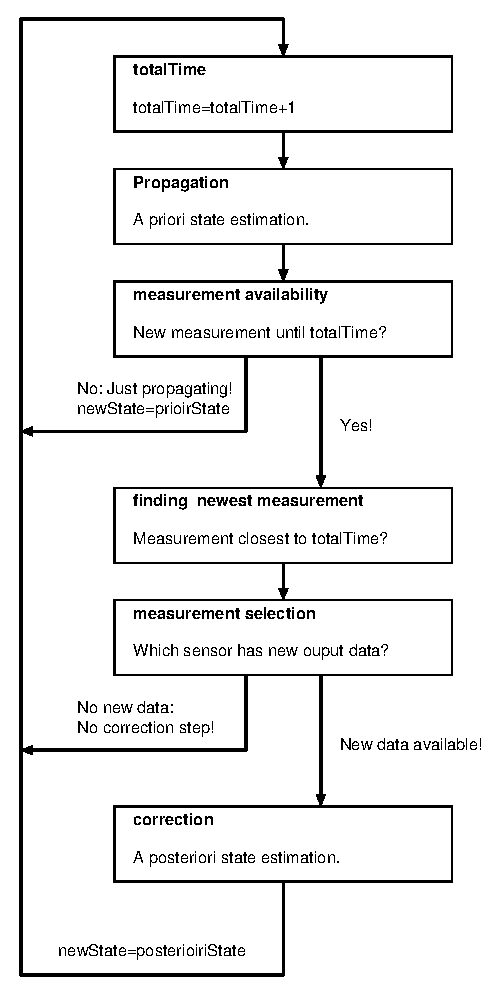
\includegraphics[width=8 cm]{pictures/structure_algo_1.eps}
\caption{The graphical represenetation of the algorithm's structure.}
\label{structure_algo}
\end{center}
\end{figure}


\begin{description}
\item[Block 1, totalTime:]
The filter estimates with constant rate the state of the system. This rate is independent on any output rate of the sensors. In the first block the time at which the state is estimated is set. It is the old time totalTime added with the constant time step t.

\item[Block 2, Propagation:]
During the second block the a priori state of the system is estimated with the help of the physical model. How and why the physical model is defined is explained in chapter \ref{state_estimation}. After this step the vector $x_{est}$ is up to date.

\item[Block 3, measurement availability:]
If there is no new measurement until the time of the a priori estimated state, the correction step is not executed. This allows the algorithm to run the ekf with a higher rate, then the IMU provide data. To summarize: If we have no new data from the sensors the system just keeps propagating based on the physical model.

\item[Block 4, finding the closest measurement:]
In this block it is searched for the closest measurement to the time of the a priori estimated state in block 2. If until the time of the estimation several sensor values are available only the newest and therefore most accurate value is taken for the correction.

\item[Block 5, measurement selection:]
Mostly not all sensors of an IMU provide an output with the same rate. Here it is tested, weather we have a new sensor value or is it still the one of the previous estimation. The correction step in block 5 is only for the new data executed. The other one still just propagate.

\item[Block 6, correction:]
As last step the correction of the a priori estimation takes place and the posteriori estimation is calculated. How the relationship between the state and the measurements look like is explained in chapter \ref{sensor_estimation}
\end{description}


\subsection*{Error Covariance}
For the measurement error covariance the noise of the different sensors are taken from the data sheets. But  they were manually scaled according to have more accurate and stable filter. For the propagation model the covariance was estimated on how accurate the equations are. But also in this case were they manually adjusted afterwards. For an easier handling only the diagonal elements have a value. The off diagonal values are all zero.

\subsection*{Jacobian Matrix}
In chapter \ref{ekf} the matrixes H and A were derived. Since the physical model and relations between state and the measurements are non linear, H and A are the Jacobian matrixes of the functions $f$ and $h$. For having an accurate as possible solution the Jacobian was in a first version calculated analytically with symbolic toolbox from MathWorks. The Jacobian matrix then has to be evaluated in every iteration step. Simulating 0.01 seconds took the filter much longer than 10 minutes. It was then decided to rewrite the algorithm calculating the Jacobian matrixes numerical. The function ekf.m [..ekfwebsite..]from MathWorks was restructured to match the requirements of this algorithm. It uses a complex step differentiation to calculate the derivatives of the function f and h [..papCompDiff..]. 


\section{State Estimation Model}\label{state_estimation}
In order to propagate the state of the system $x_{k}$ to the a priori state estimation $x^{-}_{k+1}$ the filter needs to be able to predict in what state the system will be at time $t_{k+1}$ based on its state at time $t_{k}$. In the most basic case, the assumption is that there exists no knowledge about the forces acting on the body. This leads to the so called "free mass model". However, in the case of a kite tethered to a ground station, the body is not able to move freely in three dimensions, but its movement is in a first approximation limited to a sphere with a given radius. This means, that one of the main forces acting on the body, the centripedal force, can be accounted for in the prediction. Furthermore an aerodynamical model of the kite might be able to predict also other forces than the centripedal force. In order to explore the benefits of such a model, we decided to use a spherical pendulum for the resons described in the introduction. In that case, all the forces acting on the body are known and the degrees of freedom are further reduced due to the bridled suspension. In the following sections, these two models are going to be described in detail. 

\subsection*{Free Mass Model}
The dynamics of the body are described by a system of first order differential equations describing the change in the state variables.
\begin{equation} \dot{x}=g(x,t)  \end{equation}
In this case the model is time invariant and thus g is not time dependant. 
\begin{equation} \dot{x}=g(x)  \end{equation}
Since there is no knwoledge about the forces acting on the body, this set of equation looks rather simple: 
\begin{equation} g(x)=\begin{bmatrix}  x_{4} \\  x_{5} \\ x_{6} \\ 0 \\ 0 \\ 0 \\ x_{10} \\ x_{11} \\ x_{12} \\ 0 \\ 0 \\0 \end{bmatrix} \end{equation}

\subsection*{Pendulum}
Again the dynamics are described by a system of time invariant first order differential equations. 
\begin{equation} \dot{x}=g(x)  \end{equation}
Due to the gravitation and the centripedal force being the only forces acting on the body, we can derive an exact set of differential equations that govern the motion of a spherical pendulum. Therefore we use the Euler-Lagrange-Equation to derive the differential equations as suggested in \cite[156ff]{debnath2005}.

With the kinetic energy
\begin{equation} T=\frac{1}{2}mr^2(\dot{\Theta}^2+\dot{\Psi}^2\cos^2{\Theta})  \end{equation}
and the potential energy
\begin{equation} V=-mr\sin{\Theta}  \end{equation}
the Lagrangian is defined by:
\begin{equation} L=T-V = \frac{1}{2}mr^2(\dot{\Theta}^2+\dot{\Psi}^2\cos^2{\Theta})+mr\sin{\Theta}\end{equation}

Substituting the Lagrangian into Euler-Lagrange-Equation 
\begin{equation} \frac{\partial L}{\partial \Psi}-\frac{d}{dt}\frac{\partial L}{\partial \dot{\Psi}}=0 \end{equation}
and solving for $\ddot{\Psi}$ results in:
\begin{equation} \ddot{\Psi}=2\tan{\Theta}\dot{\Theta}\dot{\Psi} \end{equation}

And similarly for $\ddot{\Theta}$:
\begin{eqnarray} \frac{\partial L}{\partial \Theta}-\frac{d}{dt}\frac{\partial L}{\partial \dot{\Theta}}=0 \\
 \ddot{\Theta}=\dfrac{\cos{\Theta}(g-r\sin{\Theta}\dot{\Psi}^2)}{r} \end{eqnarray}

The third degree of freedom, the body's rotation about its z-axis, is assumed to be constant. However, due to the convention of the euler angles, a change in phi contributes an additional term to the z component of the rotation vector in the body frame. (For further explanation see section ...) To compensate for that, the second derivative of $\Phi$ is not zero but defined as follows: 

\begin{eqnarray} \frac{d}{dt}w_{z}^{body}=\frac{d}{dt}(\dot{\Phi} - \sin{\Theta} \dot{\Psi}) =0 \\
 \ddot{\Phi}=\cos{\Theta}\dot{\Theta}\dot{\Psi}+\sin{\Theta}\ddot{\Psi} \end{eqnarray}

With the radius assumed to be constant, the fourth and eighth state variable ($r$ and $\dot{r}$) are not changing and thus their time derivatives are zero.

Therefore the set of differential equations is given by:
\begin{equation} g(x)=\begin{bmatrix} \\ x_{5} \\ x_{6} \\ x_{7} \\ 0 \\ \cos{x_{2}} \dot{x_{2}} \dot{x_{3}}+\sin{x_{2}} \ddot{x_{3}} \\  \dfrac{\cos{x_{2}}(g-r\sin{x_{2}} \dot{x_{3}}^2)}{r} \\ 2\tan{x_{2}} \dot{x_{2}} \dot{x_{3}} \\ 0  \end{bmatrix} \end{equation}

\subsection*{Solving the Differential Equations}
So far we have derived the sets of differential equations that contain all the knowledge we have about the systems. To calculate the a priori state estimation $x^{-}_{k+1}$ from the state of the system $x_{k}$ we now only need to solve these sets of differnetial equations. This is done numerically using the classical fourth-order Runge-Kutta method \cite{Kutta1901}. Note that in our case g(x) is time invariant. 
\begin{eqnarray}k_{1}&=&h g(t_{n},x_{n})\\
k_{2}&=&h g(t_{n}+\frac{1}{2}h,x_{n}+\frac{1}{2}k_{1})\\
k_{3}&=&h g(t_{n}+\frac{1}{2}h,x_{n}+\frac{1}{2}k_{2})\\
k_{4}&=&h g(t_{n}+h,x_{n}+k_{3})\\
x_{n+1}&=&x_{n} + \frac{1}{6} k_{1} + \frac{1}{3} k_{2} + \frac{1}{3} k_{3} + \frac{1}{6} k_{4} + \mathcal{O}(h^{5})\end{eqnarray}

\section{Sensor Estimation Model}\label{sensor_estimation}
An illustration of the relation between the position and velocity in $(y,x,z)$ or $(dx,dy,dz)$ and the two angles $\Phi$, $\Theta$ and $\Psi$  is shown in figure \ref{dof}. With this sketch, the assumption of a constant radius and the fact that the velocity is the derivative of the position we get to the equations: 

\begin{eqnarray}
pos\;x&=&R*cos(\Theta)cos(\Psi)\\
pos\;y&=&R*sin(\Psi)cos(\Theta)\\
pos\;z&=&R*sin(\Theta)\\
vel\;x&=&-sin(\Theta)cos(\Psi)*R*\dot{\Theta}-cos(\Theta)sin(\Psi)*R*\dot{\Psi}\\
vel\;y&=&-sin(\Theta)sin(\Psi)*R*\dot{\Theta}+cos(\Theta)cos(\Psi)*R*\dot{\Psi}\\
vel\;z&=&-cos(\Theta)*R*\dot{\Theta}\\
\end{eqnarray}
The centripetal acceleration always accting in z direction of the sensor can be calculated by the formula:
\begin{equation}
a_{cp}=\frac{v^2}{R}
\end{equation}
We then have the an additional acceleration of the earth gravitation. The earth gravitation is in the inertial frame only in z direction and has to be transformed with the $DCM_{bi}$ from the inertial in the body frame. Finally the acceleration can be written as:
\begin{equation}
acc&=& \begin{bmatrix} 0\\0\\ \frac{v^2}{R}\end{bmatrix}+DCM_{bi}*\begin{bmatrix}0\\0\\g\end{bmatrix}
\end{equation}
The magnetic field is  a constant value in Zurich. By transforming that into the body frame again with the help of the $DCM_{bi}$, the expected measurement from the magnetometer is calculated:
\begin{equation}
mag&=& DCM_{bi}* \begin{bmatrix} 0.2145 \\ 0.0060 \\ 0.4268 \end{bmatrix} [gauss]
\end{equation} 
The gyroscope measurement is directly represented by the rate of the euler angles $\dor{\Phi}$,$\dot{\Theta}$ and $\dot{\Psi}$. Since the euler angular rate has to be transformed into the body frame coordinates and additinally has a converstion about which axes is rotated the first, what the gyroscope has not,a transformation matrix has to be used as follows:
\begin{equation}
gyro=\begin{bmatrix} 1 & 0 & -sin(\Theta) \\ 0 & cos(\Phi) & sin(\Phi) cos(\Theta) \\ 0 & -sin(\Phi) & cos(\Phi)cos(\Theta) \end{bmatrix}*\begin{bmatrix} \dot{\Psi}\\ \dot{\Theta}\\ \dot{\Phi} \end{bmatrix}
\end{equation}
Because the position of the senors is not at the center of mass of the pendulum, an additional displacement vector has to be added to the position (compare figure \ref{displacement}). With transforming the distance between the center of mass and the sensor into the inertial frame, the position is adjusted. The displacement gives an additional velocity which is the crossproduct of the rate of rotation and the displacement from the center of mass. By the derivative of this additional velocity the additional acceleration is calculated. The displcement has no influence on the gyrometer measurement and the magnetometer.
\begin{figure}[h]
\begin{center}
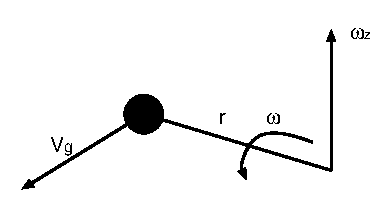
\includegraphics[width=8 cm]{pictures/displacement_1.eps}
\caption{The black dot represents the sensor, while r is the distance between the center of mass of the pendulum and the sensor.}
\label{displacement}
\end{center}
\end{figure}

